\documentclass[10pt,a4paper,twoside,openany]{memoir}

% Chapter Modifications
\usepackage{titlesec}
\titleformat{\chapter}{\normalfont\huge}{\bfseries\thechapter.}{20pt}{\bfseries\huge}

% DRAFT Watermark
\usepackage{draftwatermark}
\SetWatermarkText{DRAFT}
\SetWatermarkScale{9}
\SetWatermarkLightness{0.95}

% Version History
\usepackage{vhistory}

% Colours
\usepackage[usenames,dvipsnames,svgnames,table]{xcolor}

% Margins
\usepackage[top=2cm,bottom=3cm,inner=3cm,outer=2cm]{geometry}

% Code listings
\usepackage{listings}
\lstset{
  basicstyle=\fontfamily{lmvtt}\selectfont\small\color{black},
  columns=fullflexible,
  tabsize=3,
  frame=shadowbox
}

% Squash lists down a bit
\usepackage{enumitem}
\setlist{noitemsep}

% Links
\usepackage{hyperref}

% Font
\renewcommand*\rmdefault{cmss}

% Respect subsection numbering & sectioning depth in the TOC
\setcounter{secnumdepth}{5}
\setcounter{tocdepth}{1}

\title{CL Metaheaders \\ Open Specification \\ Revision 1.0.x}
\author{
        John Vidler \texttt{j.vidler@lancaster.ac.uk} \\
        Stephen Wattam \texttt{steve@watt.am} \\
}
\date{Compiled \today}

\begin{document}
\pagenumbering{gobble}
\maketitle

\begin{center}
\vspace*{3em}
This specification is currently under heavy development, and is incomplete in a large number of places, please ensure you use the latest edition by examining the compiled date above.

\vspace*{3em}

Comments and suggestions to be directed to\\
\texttt{j.vidler@lancaster.ac.uk} and/or \texttt{s.wattam@lancaster.ac.uk}
\end{center}

\begin{figure}[b!]
    \textit{Corpus researchers, along with many other disciplines in science are being put under continual pressure to show accountability and reproducibility in their work.
    This is unsurprisingly difficult when the researcher is faced with a wide array of methods and tools through which to do their work; simply tracking the operations done can be problematic, especially when toolchains are often configured by the developers, but left largely as a black box to the user.
    Here we present a scheme for encoding this `meta data' inside the corpus files themselves in a structured data format, along with a proof-of-concept tool to record the operations performed on a file.}
    
    \begin{flushright}
        \textit{Keeping Properties with the Data, CL-MetaHeaders-An Open Specification} \cite{vidler2017metaheaders}
    \end{flushright}
\end{figure}

\clearpage

\pagenumbering{roman}
\begin{versionhistory}
    \vhEntry{1.0.0}{}{JV|SW}{Initial draft version, bare essentials included}
    \vhEntry{1.0.1}{}{JV|SW}{Introduction of the `namespace'}
    \vhEntry{1.0.2}{}{JV|SW}{Inclusion of multiple examples, including ARFF and TEI}
    \vhEntry{1.0.3}{}{JV|SW}{Field requirements changed from `required' to optional, added in additional minimal example}
    \vhEntry{1.0.4}{20/03/2017}{JV}{Added the `history' namespace, with sub-field definitions}
    \vhEntry{1.0.5}{18/07/2017}{JV}{TBC}
\end{versionhistory}\clearpage

\setcounter{page}{0}
\pagenumbering{arabic}
\tableofcontents\clearpage

\chapter{Outline}\clearpage
\chapter{Data Formats}
\label{sec:DataFormats}

Rather than creating a new format, or trying to describe the same structure in each different document format, a single common highly portable standard was chosen.

JSON\cite{JSON}, designed to be used as a plain-text data interchange format for the web has been ported to a vast set of languages, 

\section{Data Structure}
By using JSONs \textit{object} data type, we can indefinitely nest fields within fields.
It is this feature that allows us to build tree structures using JSON, and build up complex relationships between parent and child fields.

This specification makes extensive use of this mechanism to provide conflict-less field-name spaces in to which tools and libraries can have relatively free rein to define their own structures.

\begin{figure}[ht!]
    \centering
    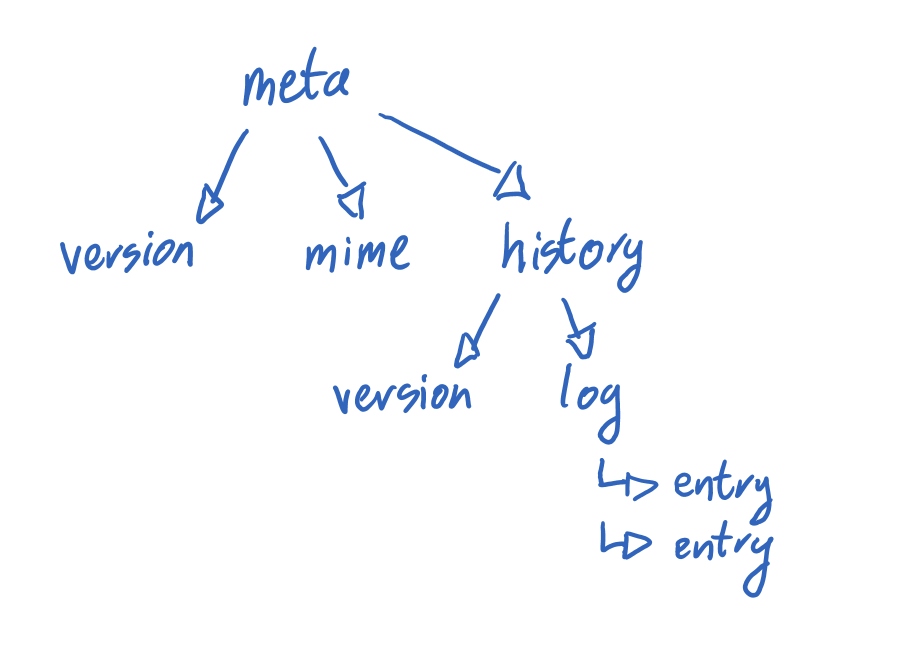
\includegraphics[width=0.5\textwidth]{diagrams/meta-tree.png}
    \caption{An example of the tree-structure JSON affords the metaheader specification}
    \label{structure:meta-tree}
\end{figure}

\section{Semantic Versioning}
\label{sec:SemanticVersioning}
Semantic version fields, denoted by the \texttt{\_\_version\_\_} field name use string format values, but must strictly follow the Semantic Versioning (SemVer) scheme of \texttt{major.minor.patch}, as a dotted-triple\footnote{`Dotted-Triple' - A sequence of three independent sub items separated by a dot, usually numeric, but not required to be, and if numeric, multiple number bases can be used in separated sections.} as defined in the latest draft of the specification.

The three sections of the semantic version field are (currently, at the time of writing according to semver 2.0.0) defined as follows:
\begin{enumerate}
    \item[major] Version when you make incompatible API changes,
    \item[minor] Version when you add functionality in a backwards-compatible manner, and
    \item[patch] Version when you make backwards-compatible bug fixes.
\end{enumerate}

It should be noted that the \texttt{minor} and \texttt{patch} fields must only increment if the changes made are backward-compatible with the previous versions. 
If they are not, then the \texttt{major} version should tick over and reset the other two to indicate the break in compatibility.

The current draft format for semantic versioning can be found at \url{http://semver.org/}\clearpage
\chapter{Recognised Fields}
The preliminary set of features identified for inclusion have been selected to allow the identification of key features of the subsequent texts, and allow them to be correctly loaded by software, and are:

\begin{itemize}
    \item common to all machine-readable text representations;
    \item necessary-yet-uninteresting features of the dataset;
    \item generally useful across many tool types.
\end{itemize}



\section{\texttt{\_\_version\_\_}}
\textit{(Optional, String)}

The specification version that this header complies with, if missing, assumes the latest draft.
Version numbers are specified following Semantic Versioning \cite{semver}, making it easy to determine compatibility.


\section{\texttt{encoding}}
\textit{(Optional, String)}

Character encoding of current text, as defined by the IANA list of preferred text encoding names\cite{EncodingNames}.
While optional, it is strongly advised that this field be present to avoid any ambiguity in parsing.
If absent, this implicitly defaults to UTF-8.

\section{\texttt{mime}}
\textit{(Optional, String)}

The extended MIME\cite{MIMETypes} type used to describe what this file is.


\section{\texttt{group}}
\textit{(Optional, String or Object)}

Used to track which files belong to collections, defined as an object conforming to the \texttt{group} namespace specification.\clearpage
\chapter{Namespaces}

Namespaces extend the basic meta block with additional functionality.
Developers are encouraged to create their own namespace for their own tool(s) if none of the currently accepted namespaces listed here apply.

To petition to have your namespace officially accepted, contact should be made through raising an issue at \url{https://github.com/UCREL/CL-metaheaders/issues} with a new feature request listing the following features of the proposed new namespace:

\begin{enumerate}
    \item The top-level name, as it should appear in the header
    \item Any field names that are included
    \item The current latest version, in Semantic Version\cite{semver} format
    \item The name contact details for the current maintainer
\end{enumerate}

Along with a clear description of what the namespace is used for, and any other details the submitter feels necessary.

If there is a specific tool or set of tools that uses the namespace described, details should be given of what the tool does, along with where the tool can be found, ideally as a web link to a stable address (GitHub pages are one such example, where the project URL is unlikely to change, but other sites are also acceptable).

\vspace{3em}\hrule\vspace{3em}

The rest of this section is given over to concrete implementations of namespaces recognised as 'standard' by this specification.
If you are planning to propose additional namespaces be added to the specification, the \texttt{history} namespace can be viewed as a template for the format and general content of your addition.

\clearpage\section{\texttt{history} - Operations History}

\begin{tabular}{r|l}
    Maintainer & John Vidler (\href{mailto:j.vidler@lancaster.ac.uk}{j.vidler@lancaster.ac.uk}) \\
    Version & 1.0.0 \\
    Last Updated & 12 June 2017 \\
\end{tabular} \vspace{1em}

A top-level namespace conforming to the \texttt{history} namespace specification that describes the processing history of this file. Complies with the interface specification and thus has an inner \texttt{\_\_version\_\_} field.

The complete structure for the \texttt{history} namespace is as follows (newlines inserted for clarity, and values skipped for brevity):

\begin{lstlisting}
{
    "__version__": "1.0.0",
    "log": [
        { "binary": "...", "time": "...", "args": "...", "platform": "...", "md5": "..." },
        { "binary": "...", "time": "...", "args": "...", "platform": "...", "md5": "..." }
    ]
}
\end{lstlisting}

Note that the $log$ field is an array of operations, which may contain any number of entries, including zero.


\subsection{\texttt{\_\_version\_\_}}
(String, Required)

The SemVer (see \ref{sec:SemanticVersioning}) compliant version that this history meta-block complies with, currently at 1.0.0.


\subsection{\texttt{log}}
(Array, Optional)

The array of logged actions, each entry should be a log-object.
If this field is absent, compliant parser implementations should interpret this as a zero-length array (no logged actions).
Each object in this array should have at least a $binary$ and $time$ field, but may also optionally include $args$, $platform$, and $md5$ fields as required.

\textbf{NOTE:} The log entries are likely to be an in-time-order array, but if you require guaranteed true time-order listing, ensure the parsing application sorts by the $time$ field.

\subsubsection{\texttt{binary}}
(String, Required)

The binary executed on this file.
If possible, non-system specific paths should be used to aid with compatibility between platforms.

\subsubsection{\texttt{time}}
(String, Required)

An ISO8601\cite{ISO/8601} format string for when the binary was executed.

\subsubsection{\texttt{args}}
(String, Optional)

Any command-line arguments that were passed to the binary for this log entry.
Quotes must be escaped in the string to comply with the JSON specification.

\subsubsection{\texttt{platform}}
(String, Optional)

The dot-delimited platform and architecture that this command was executed on.
Examples of possible values are shown below, but any valid $platform.arch$ string is permissible.

\begin{itemize}
    \item{Linux.x86}
    \item{Linux.x64}
    \item{Linux.ARMv7LE}
    \item{Linux.ARMv7BE}
    \item{Windows.x86}
    \item{Windows.x64}
    \item{osX.x86}
    \item{osX.x64}
\end{itemize}


\subsubsection{\texttt{md5}}
(String, Optional)

The MD5 hash string of the binary executed for this log entry.


\section{Example}

\lstinputlisting{examples/ns-history/example-json.json}

\noindent\textit{(NOTE: Linebreaks, indentation, and spacing added for readability but not required for the header to function)}\clearpage
\chapter{Embedding}

\section{JSON}
JSON has no comment format, but is our native storage type, so a simple $``meta'':\{ ... \}$ inside the top-level object provides the entry point for the meta header.
In the (unlikely) event that the field ``meta'' is already used by the format in question, the alternative form $``\_\_meta\_\_''$ should be used.
Parsers working with `bare' JSON like this should attempt to read both types of block, and pick the one with a $\_\_version\_\_$ field if there is any ambiguity.

This is the only format that the meta header is \textit{not} inside a comment field, at present.

\section{WEKA ARFF}
Uses \% for comments, must be the first character on the line (may or may not ignore whitespace before \%).
The most direct way to include a meta header to this format is to simply encode the entire thing on one line to avoid parsing additional lines prefixed by \%`s.
However, to maintain readability, these will be supported in the finalised 1.0 specification.

To identify the meta header in among any other comments, the opening comment should be formatted thus; $\%!meta {...}$ and if the meta block spans multiple comment lines, only the first one should have the $!meta$ identifier.

\section{XML}
Uses the $<!-- ... -->$ format for comments, and can be placed anywhere, but some XML parsers might not support this and complain if the comment is the first thing in the file--incorrectly identifying the file as having multiple roots, despite not actually being a root element.
Rather than mandate that tools should update their parsers, we allow the following format anywhere in the first block of the file; $<!-- meta \{ ... \} -->$ wherein the standard then uses the normal JSON formatted data, and can span multiple lines.

\clearpage
%\chapter{Tools}

\section{Meta}\clearpage
%\chapter{Libraries}

\section{JavaScript}

\section{Java}

\section{Python}

\section{Ruby}\clearpage
\chapter{Examples}
The following sections demonstrate some example embedded meta entries in various file types.

If you have an additional file type example that is missing in this section, post a minimum-demonstrating-example as an issue at \url{https://github.com/UCREL/CL-metaheaders/issues} either as a plain request, or as a pull request for this document to be merged in.

\section{Absolute Minimal Header}
This example shows the absolute minimal header embedded in a TEI XML file.
The contents of the actual TEI tag have been omitted, as they serve no purpose in demonstrating the header.
\lstinputlisting{examples/minimum.xml}

\section{Valid JSON}
\lstinputlisting{examples/json-valid.json}

\section{Valid ARFF}
This example has been truncated, as it is substantially long, and the metaheader is near the top of the file.
\lstinputlisting[lastline=15]{examples/titanic.arff}

\section{Valid TEI XML}
\lstinputlisting{examples/tei-valid.xml}\clearpage

\bibliographystyle{plain}
\bibliography{papers,software,standards,surveys}

\end{document}